\documentclass[12pt,a4paper]{report}
\usepackage[utf8]{inputenc}
\usepackage[english]{babel}
\usepackage{amsmath}
\usepackage{amsfonts}
\usepackage{amssymb}
\usepackage{graphicx}
\usepackage{eurosym}
\usepackage[left=2cm,right=2cm,top=2cm,bottom=2cm]{geometry}
\usepackage{wrapfig}
\usepackage{mathdots}
\usepackage{caption}
\usepackage{cite}
\usepackage{mathrsfs}
\usepackage{float}
\author{Communications department}
\title{Ground Station localization}

\begin{document}
\maketitle

\begin{figure}[H]
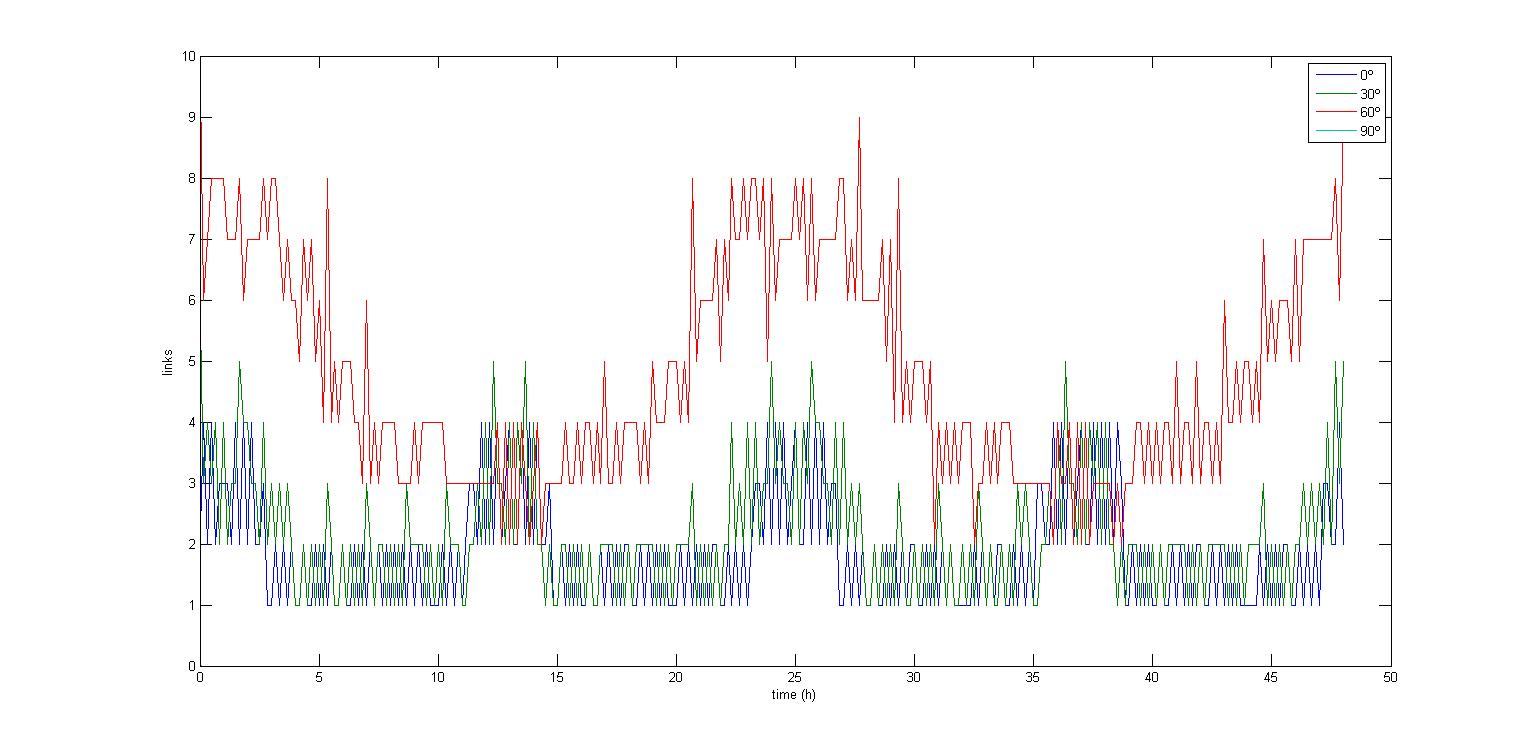
\includegraphics[scale=0.3]{0_30_60_90_nd.jpg}
\caption{Links vs time for latitudes from 0º to 90º in a non intercalated configuration}
\end{figure}

\begin{figure}[H]
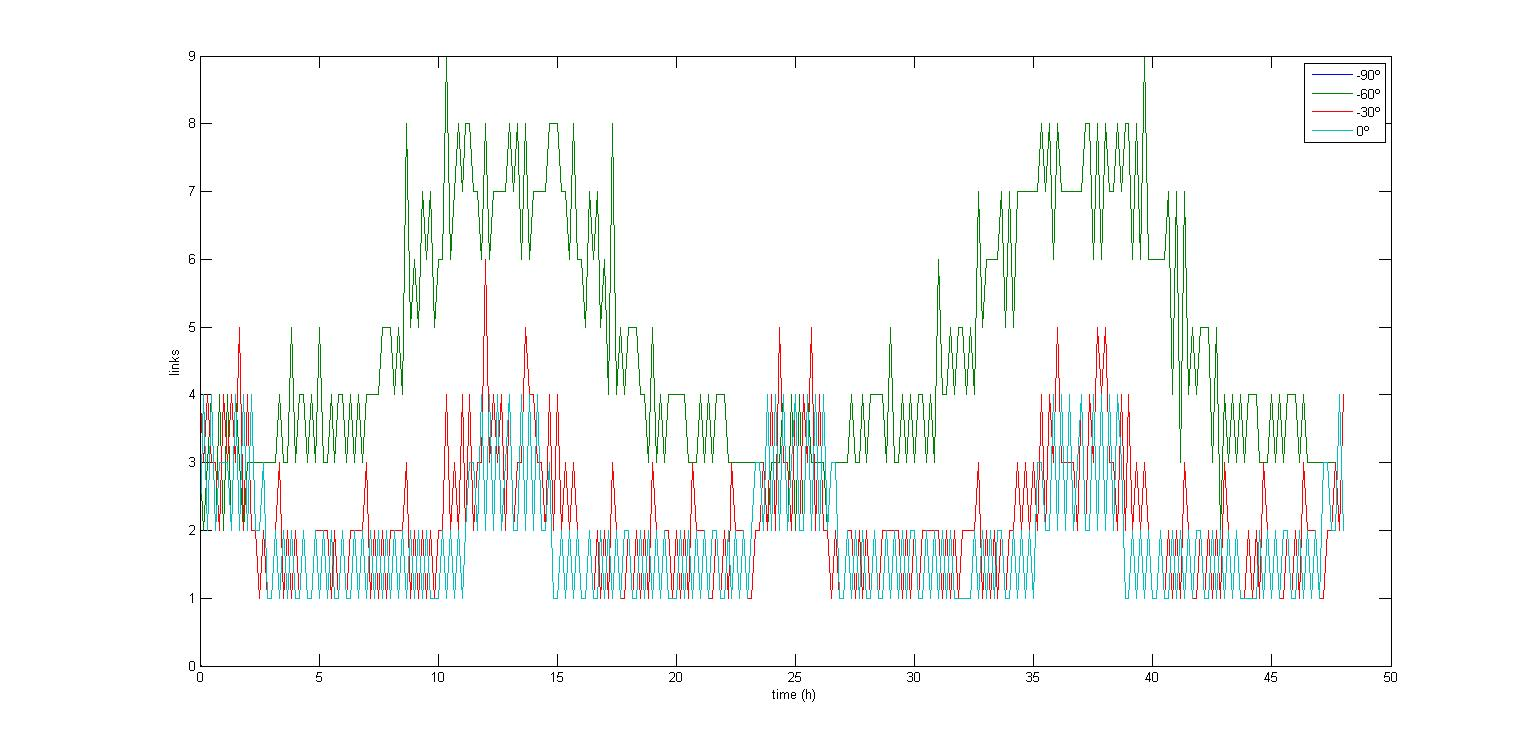
\includegraphics[scale=0.3]{-90_-60_-30_0_nd.jpg}
\caption{Links vs time for latitudes from -90º to 0º in a non intercalated configuration}
\end{figure}

\begin{figure}[H]
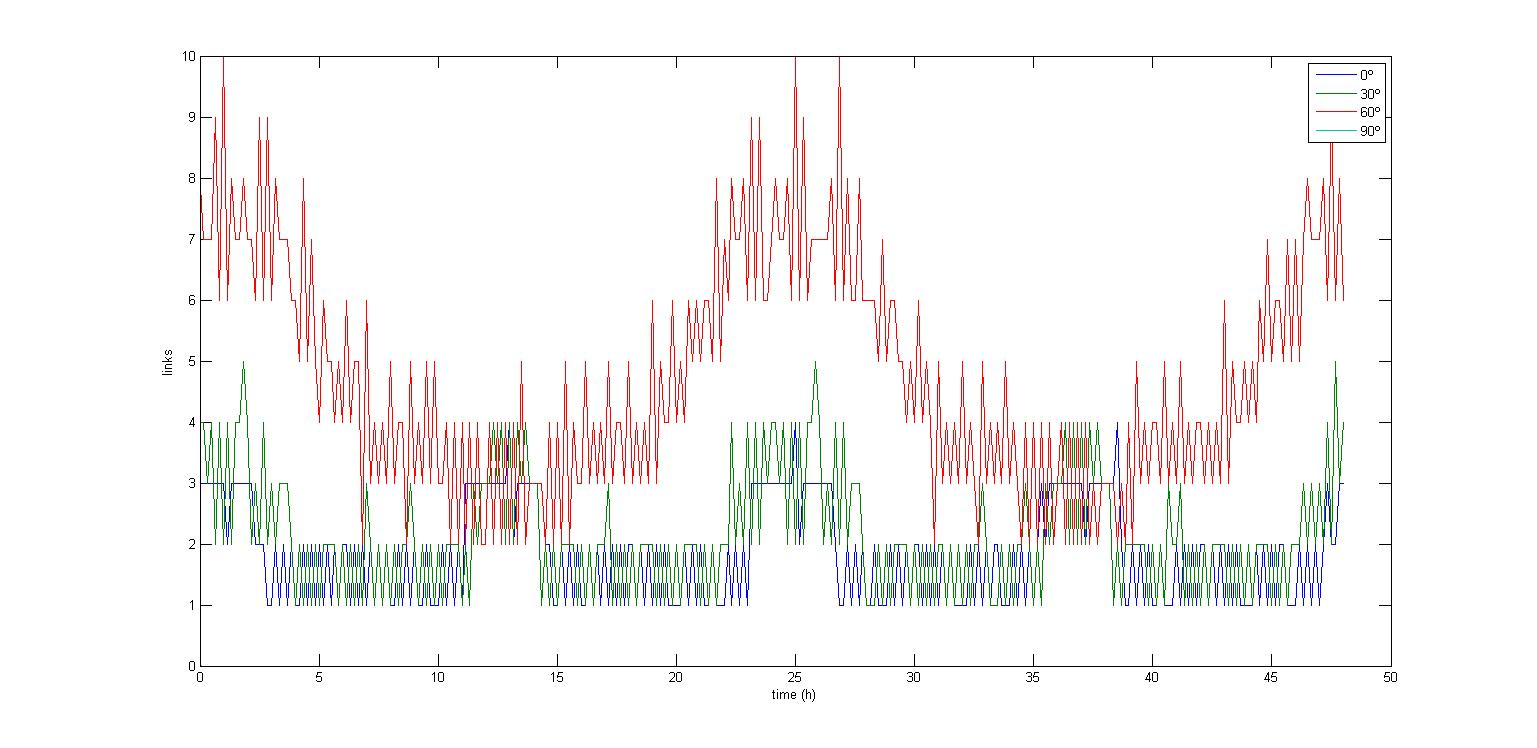
\includegraphics[scale=0.3]{0_30_60_90_d.jpg}
\caption{Links vs time for latitudes from 0º to 90º in an intercalated configuration}
\end{figure}

\begin{figure}[H]
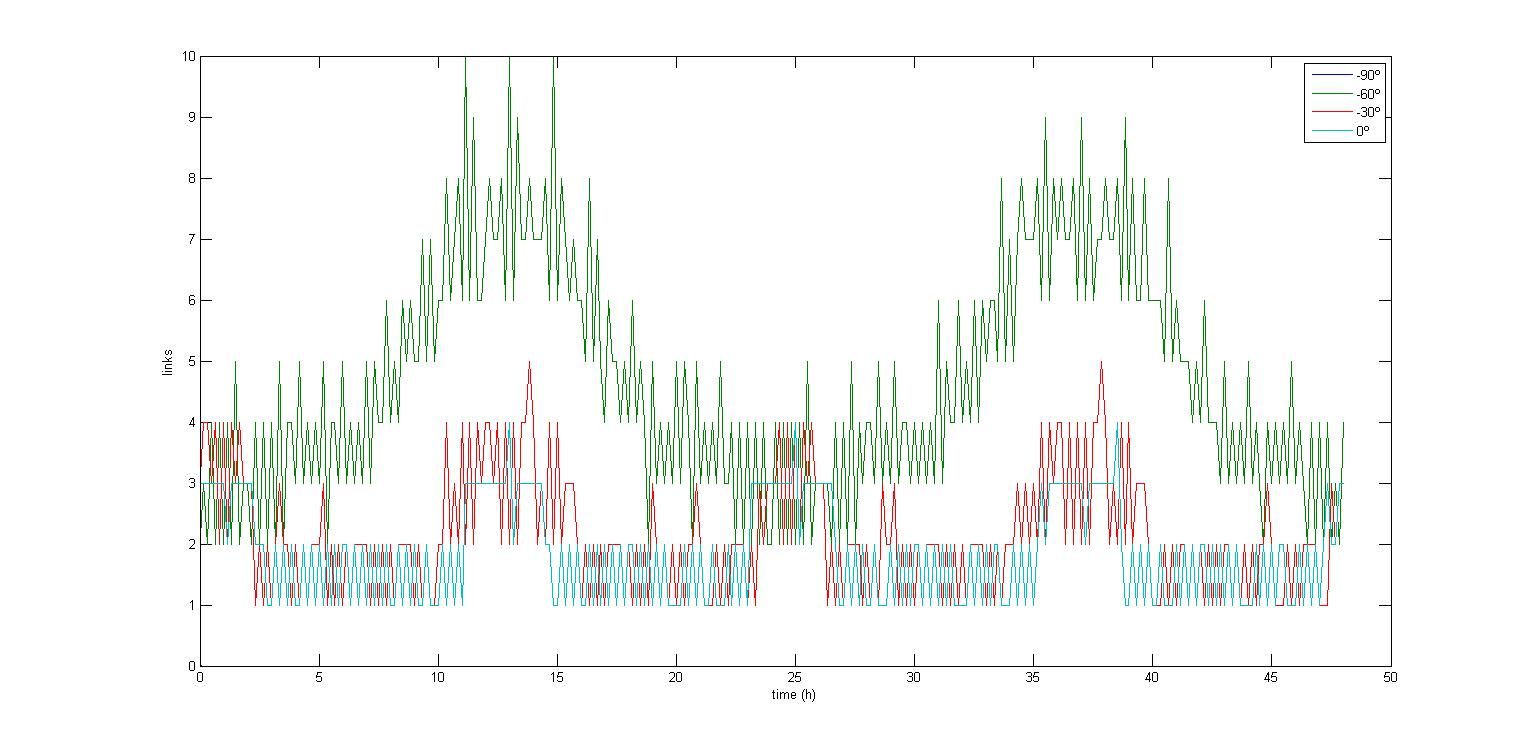
\includegraphics[scale=0.3]{-90_-60_-30_0_d.jpg}
\caption{Links vs time for latitudes from -90º to 0º in an intercalated configuration}
\end{figure}

\begin{figure}[H]
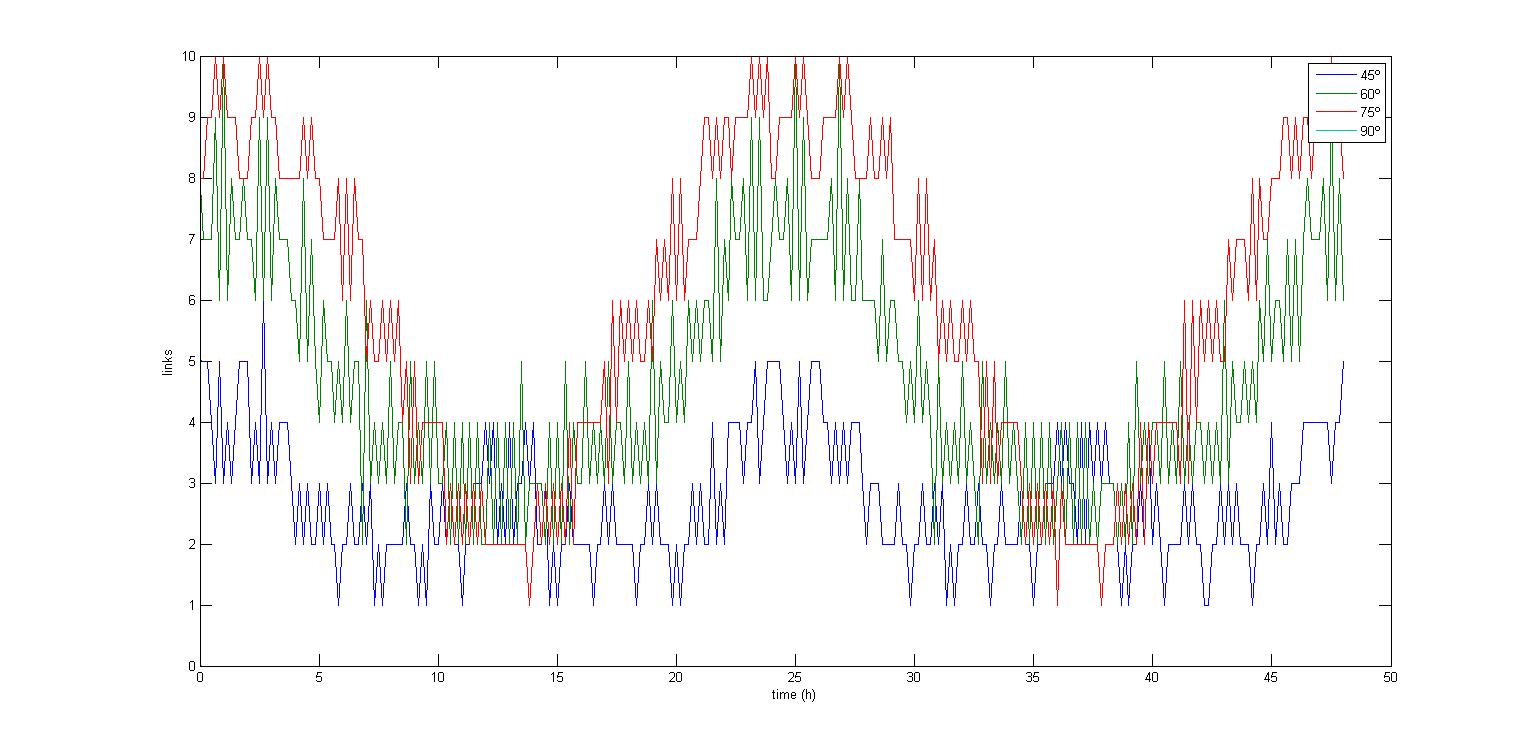
\includegraphics[scale=0.3]{45_60_75_90_d.jpg}
\caption{Links vs time for latitudes from 45º to 90º in a intercalated configuration}
\end{figure}

\begin{figure}[H]
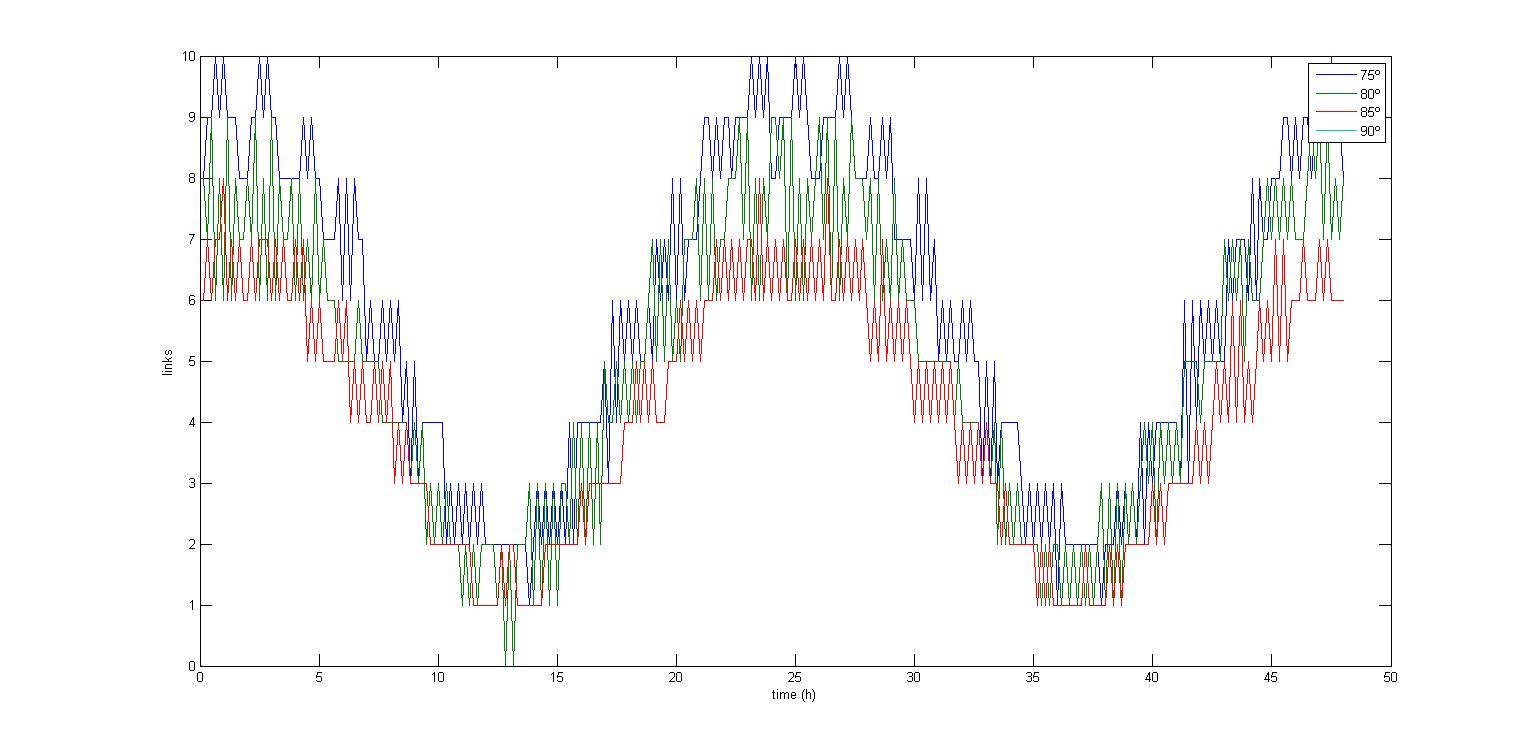
\includegraphics[scale=0.3]{75_80_85_90_d.jpg}
\caption{Links vs time for latitudes from 75º to 90º in a non intercalated configuration}
\end{figure}

\begin{figure}[H]
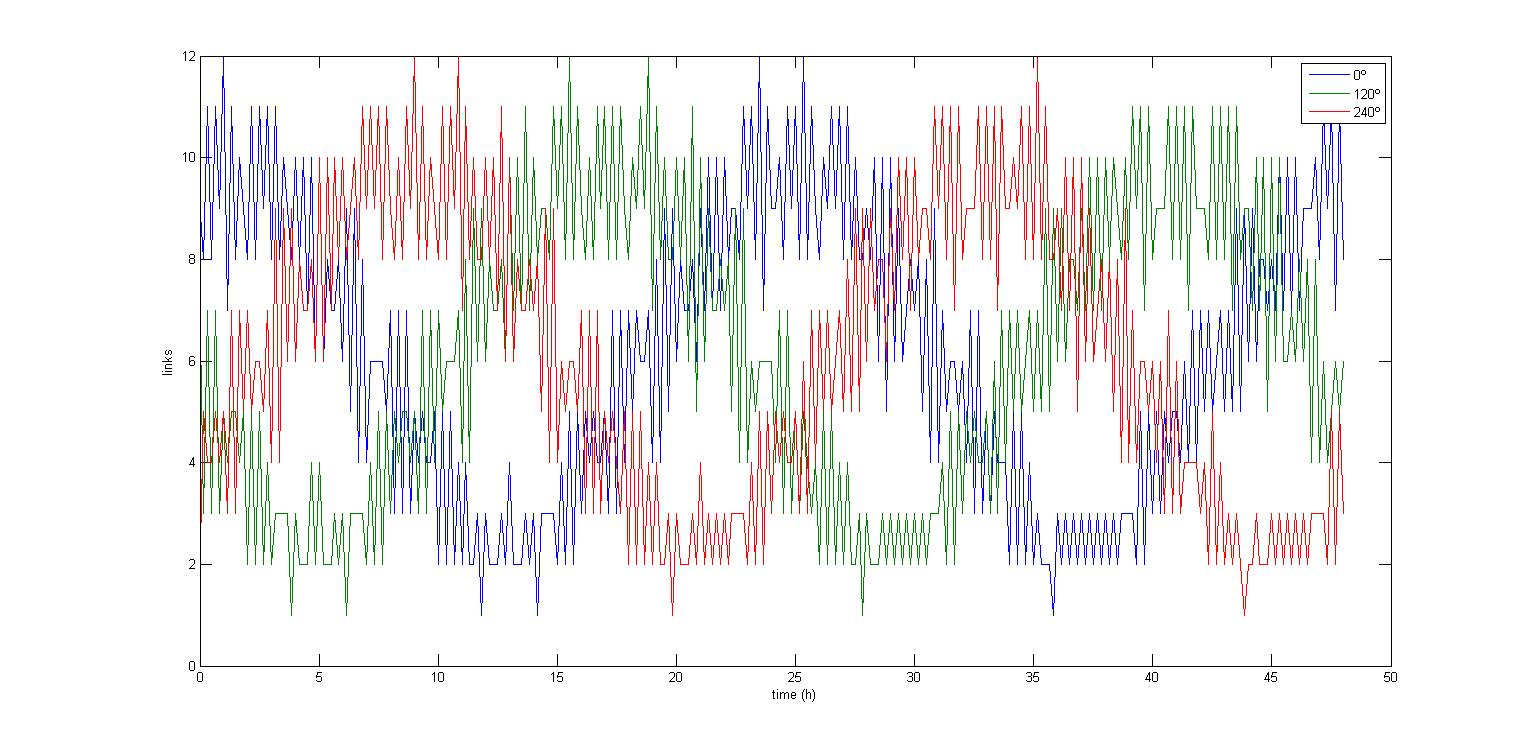
\includegraphics[scale=0.3]{0_120_240_long.jpg}
\caption{Links vs time for latitudes from 75º to 90º in a non intercalated configuration}
\end{figure}

\end{document}